\documentclass[11pt,a4paper,notitlepage,fleqn]{article}
\usepackage[T1]{fontenc}
\usepackage{graphicx}
\usepackage{url}
\usepackage{gensymb}
\title{Thermal Diffusion Final Report}
\author{Jonathan Cadman}
\begin{document}
	\maketitle
	\section{Introduction}
	My research this semester was a continuation of previous work by others on the topic of thermal diffusion. The part that I contributed to was the creation of new testing setups, utilizing different materials than previous experiments. In former years, although simulations for other materials were run, none had been done. Thus, I created rod setups using both aluminum, which would likely have similar results to the copper used in the past, and stainless steel, which we hoped would have vastly different results. We were curious if due to the slower nature of the diffusion in stainless steel, that it might get rid of some of the various factors that had been thrown in, such as the z\textsubscript{eff}, or that the rod needed to be represented as 22 cm\footnote{I will be referencing the size of the rods by the section that is outside of the heat sinks. This will mean the 20cm rod I talk about will actually be 22cm (1cm on each side to fit the sinks), and the 10cm rod will actually be 12cm.} long in the modeling for fit. I also contributed to the code, and fixed a small bug that was causing issues and not properly creating the heater in rod's array. Additionally, a decent amount of my time was spent creating models of what the rods were likely to behave like once created, which influenced our choice of rod length. Once the creation of the rods was complete, I moved on to also taking data, and attempting to fit it with the numerical model.
	\section{Procedure}
	\subsection{Modeling}
	\begin{figure}
		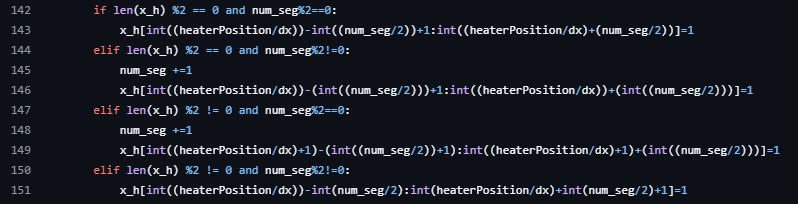
\includegraphics[width=\textwidth]{EditedCode.png}
		\caption{The code here shows the method of placing the heater in the rod array, with the 150 and 151st lines being my addition.}
		\label{Figure 1}
	\end{figure}
	\begin{figure}
		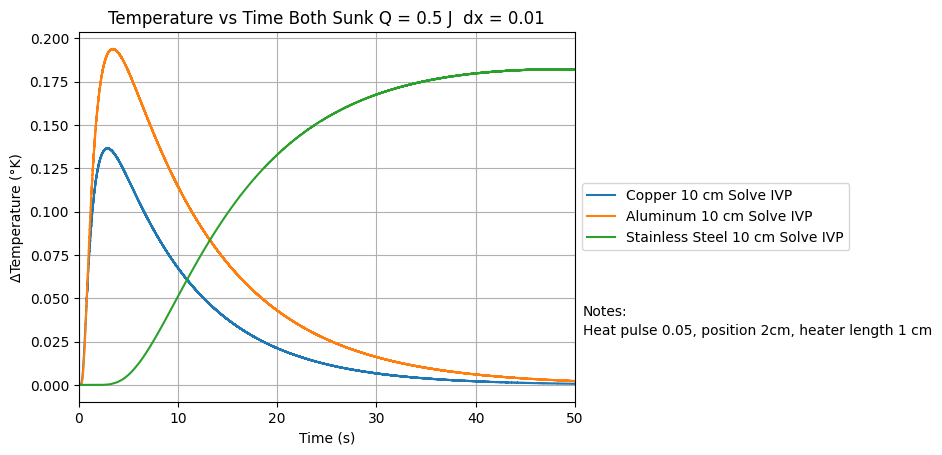
\includegraphics[width=\textwidth]{../../Thermal-Diffusion/Graphs/HighRes(dx less than or eq 0.015)/Copper_vs_Aluminum_10cm_bothsunk.png}
		\caption{This graph shows the diffusion of 3 different materials of rods. All of the rods are 10cm long, have a heater length of 1 cm in the center of the rod, are using a heat pulse of 0.05 seconds, and measuring at 2cm.}
		\label{Figure 2}
	\end{figure}
	\begin{figure}
		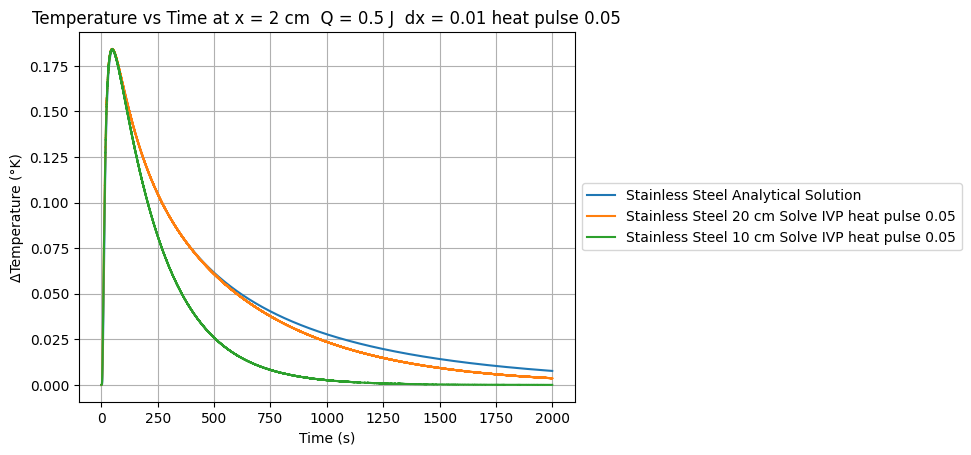
\includegraphics[width=\textwidth]{../../Thermal-Diffusion/Graphs/HighRes(dx less than or eq 0.015)/Stainless_Steel_20cm_10cm_higherres_2000.png}
		\caption{This graph shows the diffusion of 2 stainless steel rods, one 10cm and the other 20cm.}
		\label{Figure 3}
	\end{figure}
	One of the first things I was tasked with was creating models of the rods that we were intending to test. I set up a GitHub repository in order to keep track of not only the code changes that I was making, but also so that I could have a way of making my graphs and supporting code public if anyone should desire to look at them in the future. The repository is at \url{https://github.com/JMan14159/IC-Thermal-Diffusion-2026}. I started by reproducing a figure in the previous paper comparing how the different materials diffused heat at a set position and length of rod. Then, using the same solve IVP method, I added an additional line to the graph using the thermal properties of stainless steel, to compare how it behaves relative to the previously tested copper rods. From this, we were able to see that a 20cm stainless steel rod would take significantly longer than a 20cm copper rod, by a factor of around 18 times longer. This means that a 20cm stainless steel rod takes about 3500 seconds whereas a copper rod would take around 200 seconds for the same heat pulse. From this information we were able to make the informed decision to use a shorter 10cm rod for some of our data taking, as the 20cm takes a long time to gather data. In the process of this modeling I noticed a different in the peak temperature of the numerical model compared to the solve IVP method. I trialed different changes and found that if we increased the precision of the model by adjusting the dx I could eliminate this difference. When messing around with those values I found there was a bug in the code that would mean the heater never got added to the array of the rod. This bug was due to a series of if and elif statements, which left out one case, and I added the missing case to appropriately place the heater in the array, as shown in Figure \ref{Figure 1}. A sample of the models that I made can be seen in Figures \ref{Figure 2} and \ref{Figure 3}.
	\newpage
	\subsection{Setting up the rods}
	\subsubsection{Housing}
	\begin{figure}
		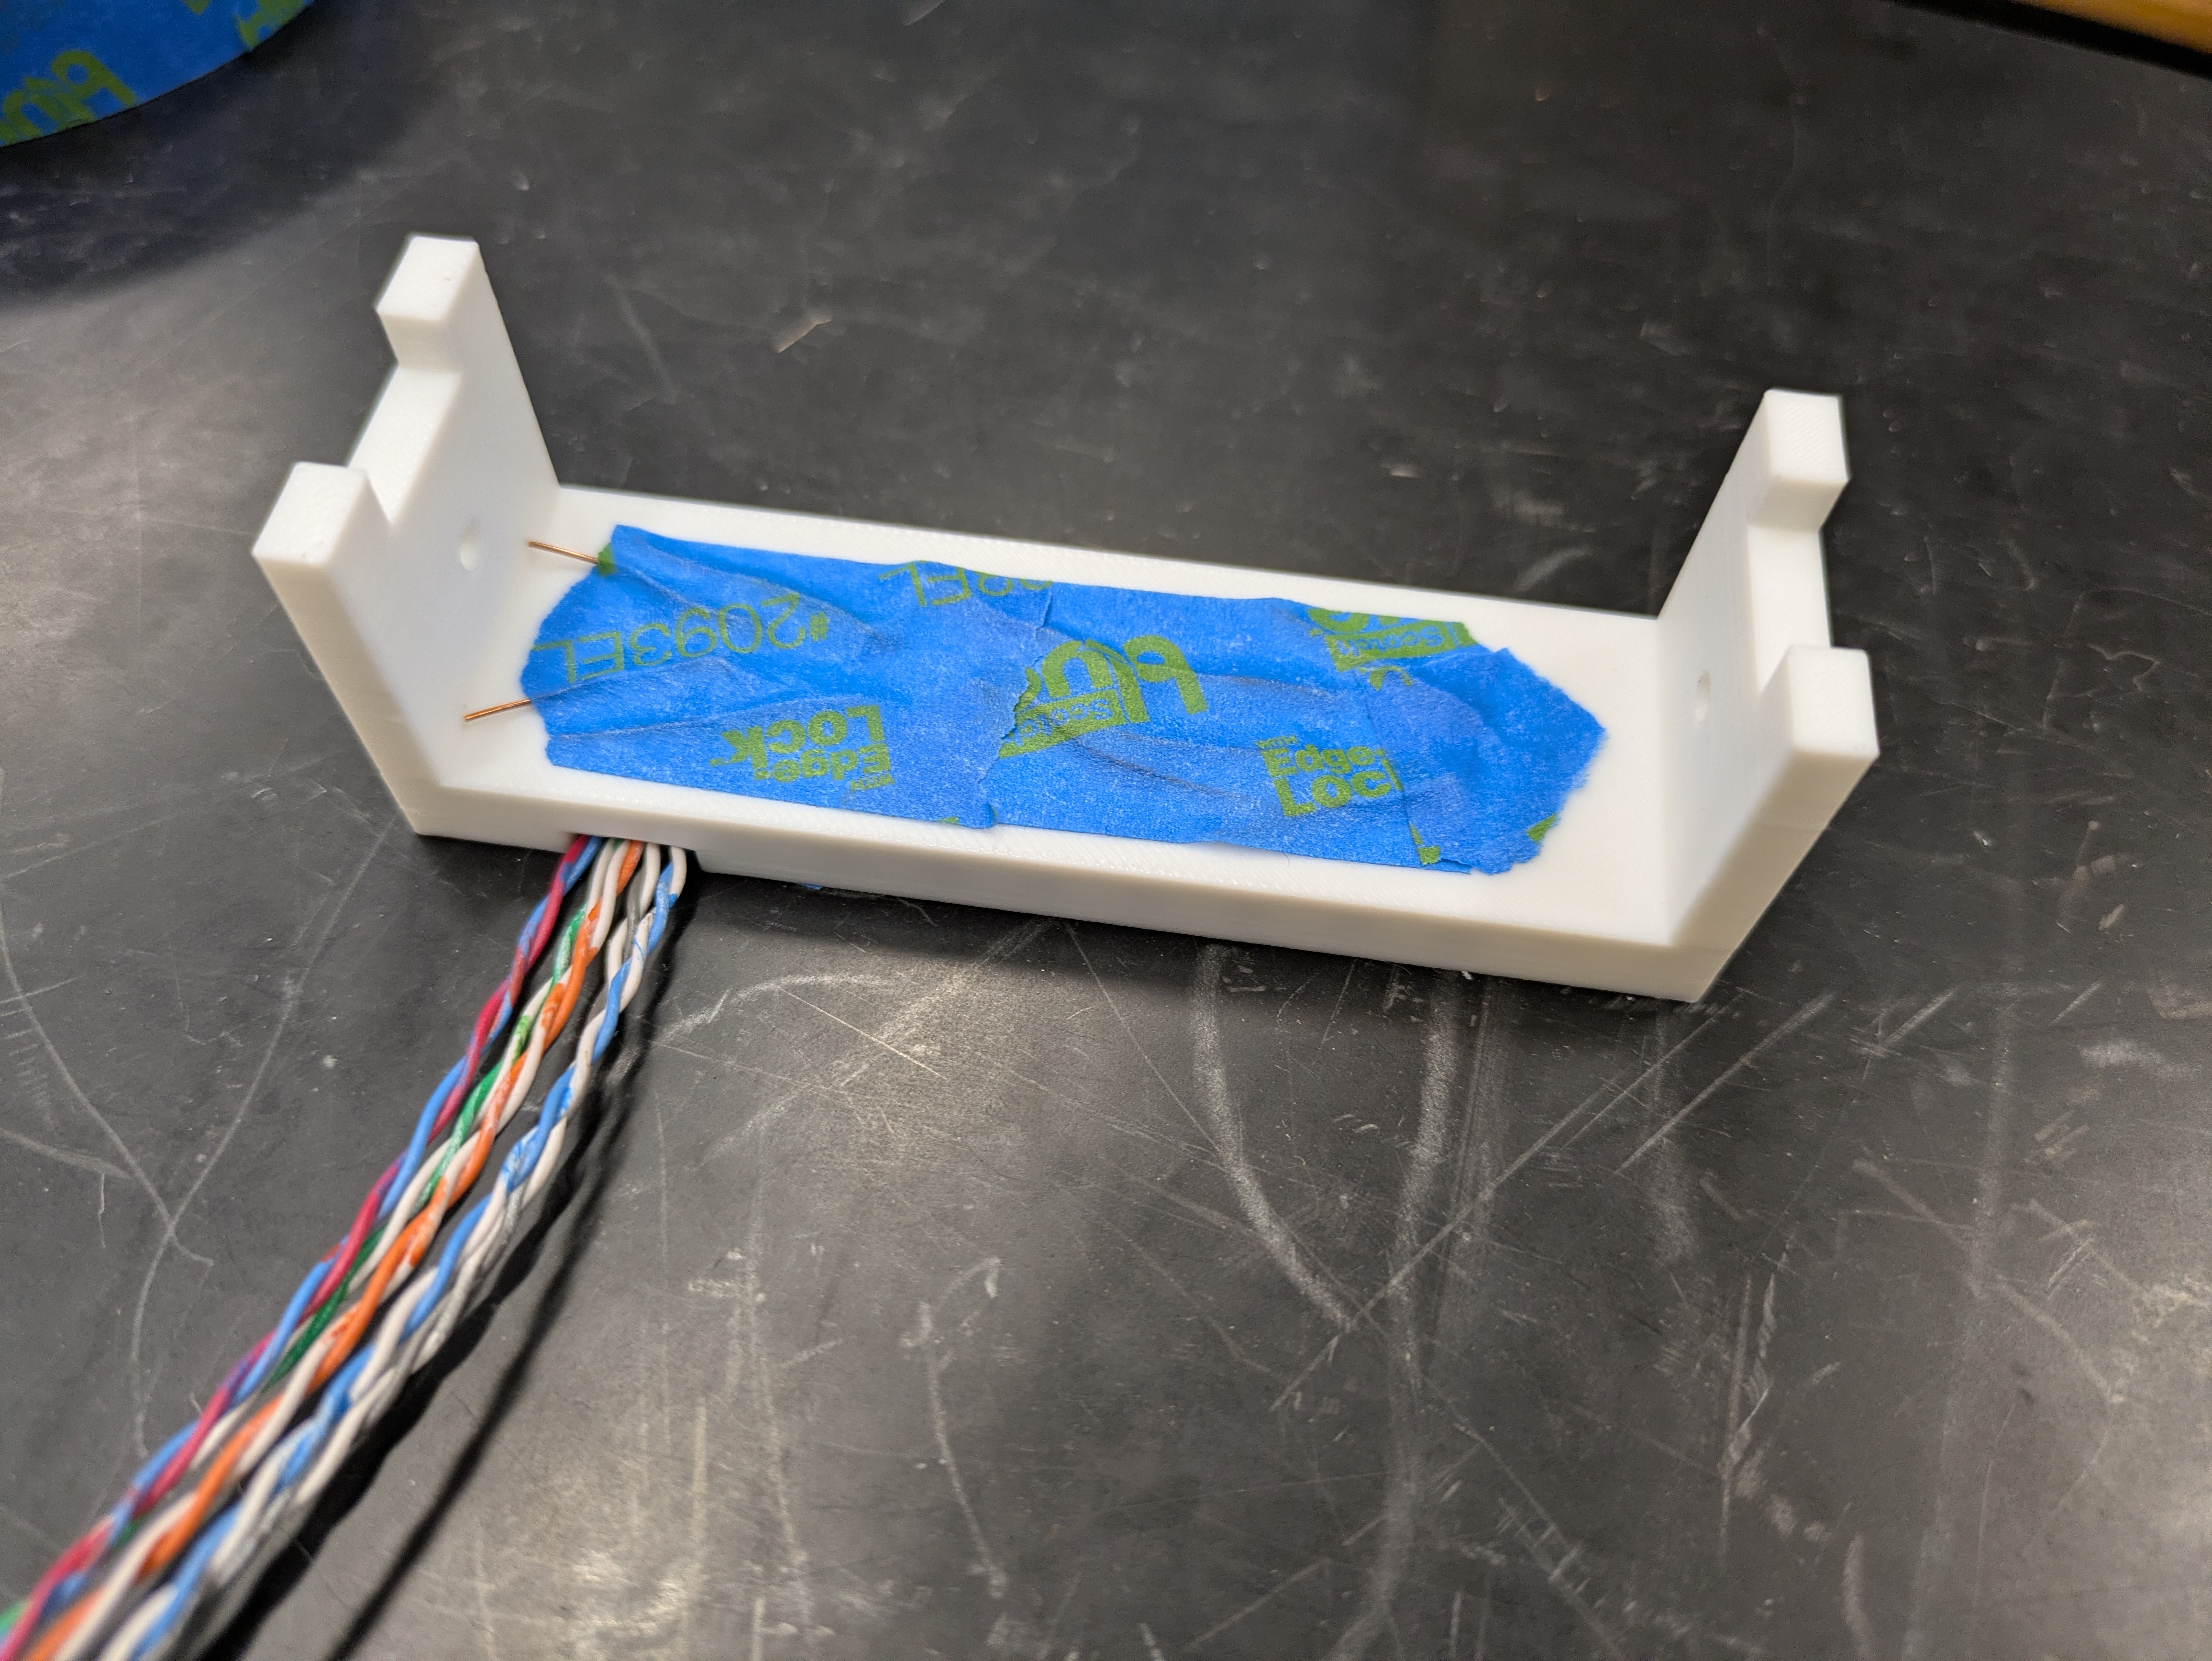
\includegraphics[width=\linewidth,trim={0 28cm 0 10cm},clip]{PXL_20260305_161435084.jpg}
		\caption{Shown here is one of the 10cm rod housings, with the wires run through and bottom glued on.}
		\label{Housing}
	\end{figure}
	In order to accommodate the shorter 10cm rods, we needed a new housing to hold the rod of the appropriate length. Not only was this new housing made shorter in length, but the holes for the wires to pass through and the rod to fit in were also made smaller. Once we had the 3D printed housings, it was my job to take old telephone wires, wrap the pairs together, and thread them through the holes in housing's base. Once all the wires were set in place with enough wire entering the main space of the housing, they were glued shut with epoxy. The top bit of the wire in the housing was then stripped and bent into the shape of a loop, to help with soldering in the future. This was done for 3 different setups, 2 of which were designed for 10cm rods, and the other for a 20cm rod.
	\subsubsection{Heater}
	\begin{figure}
		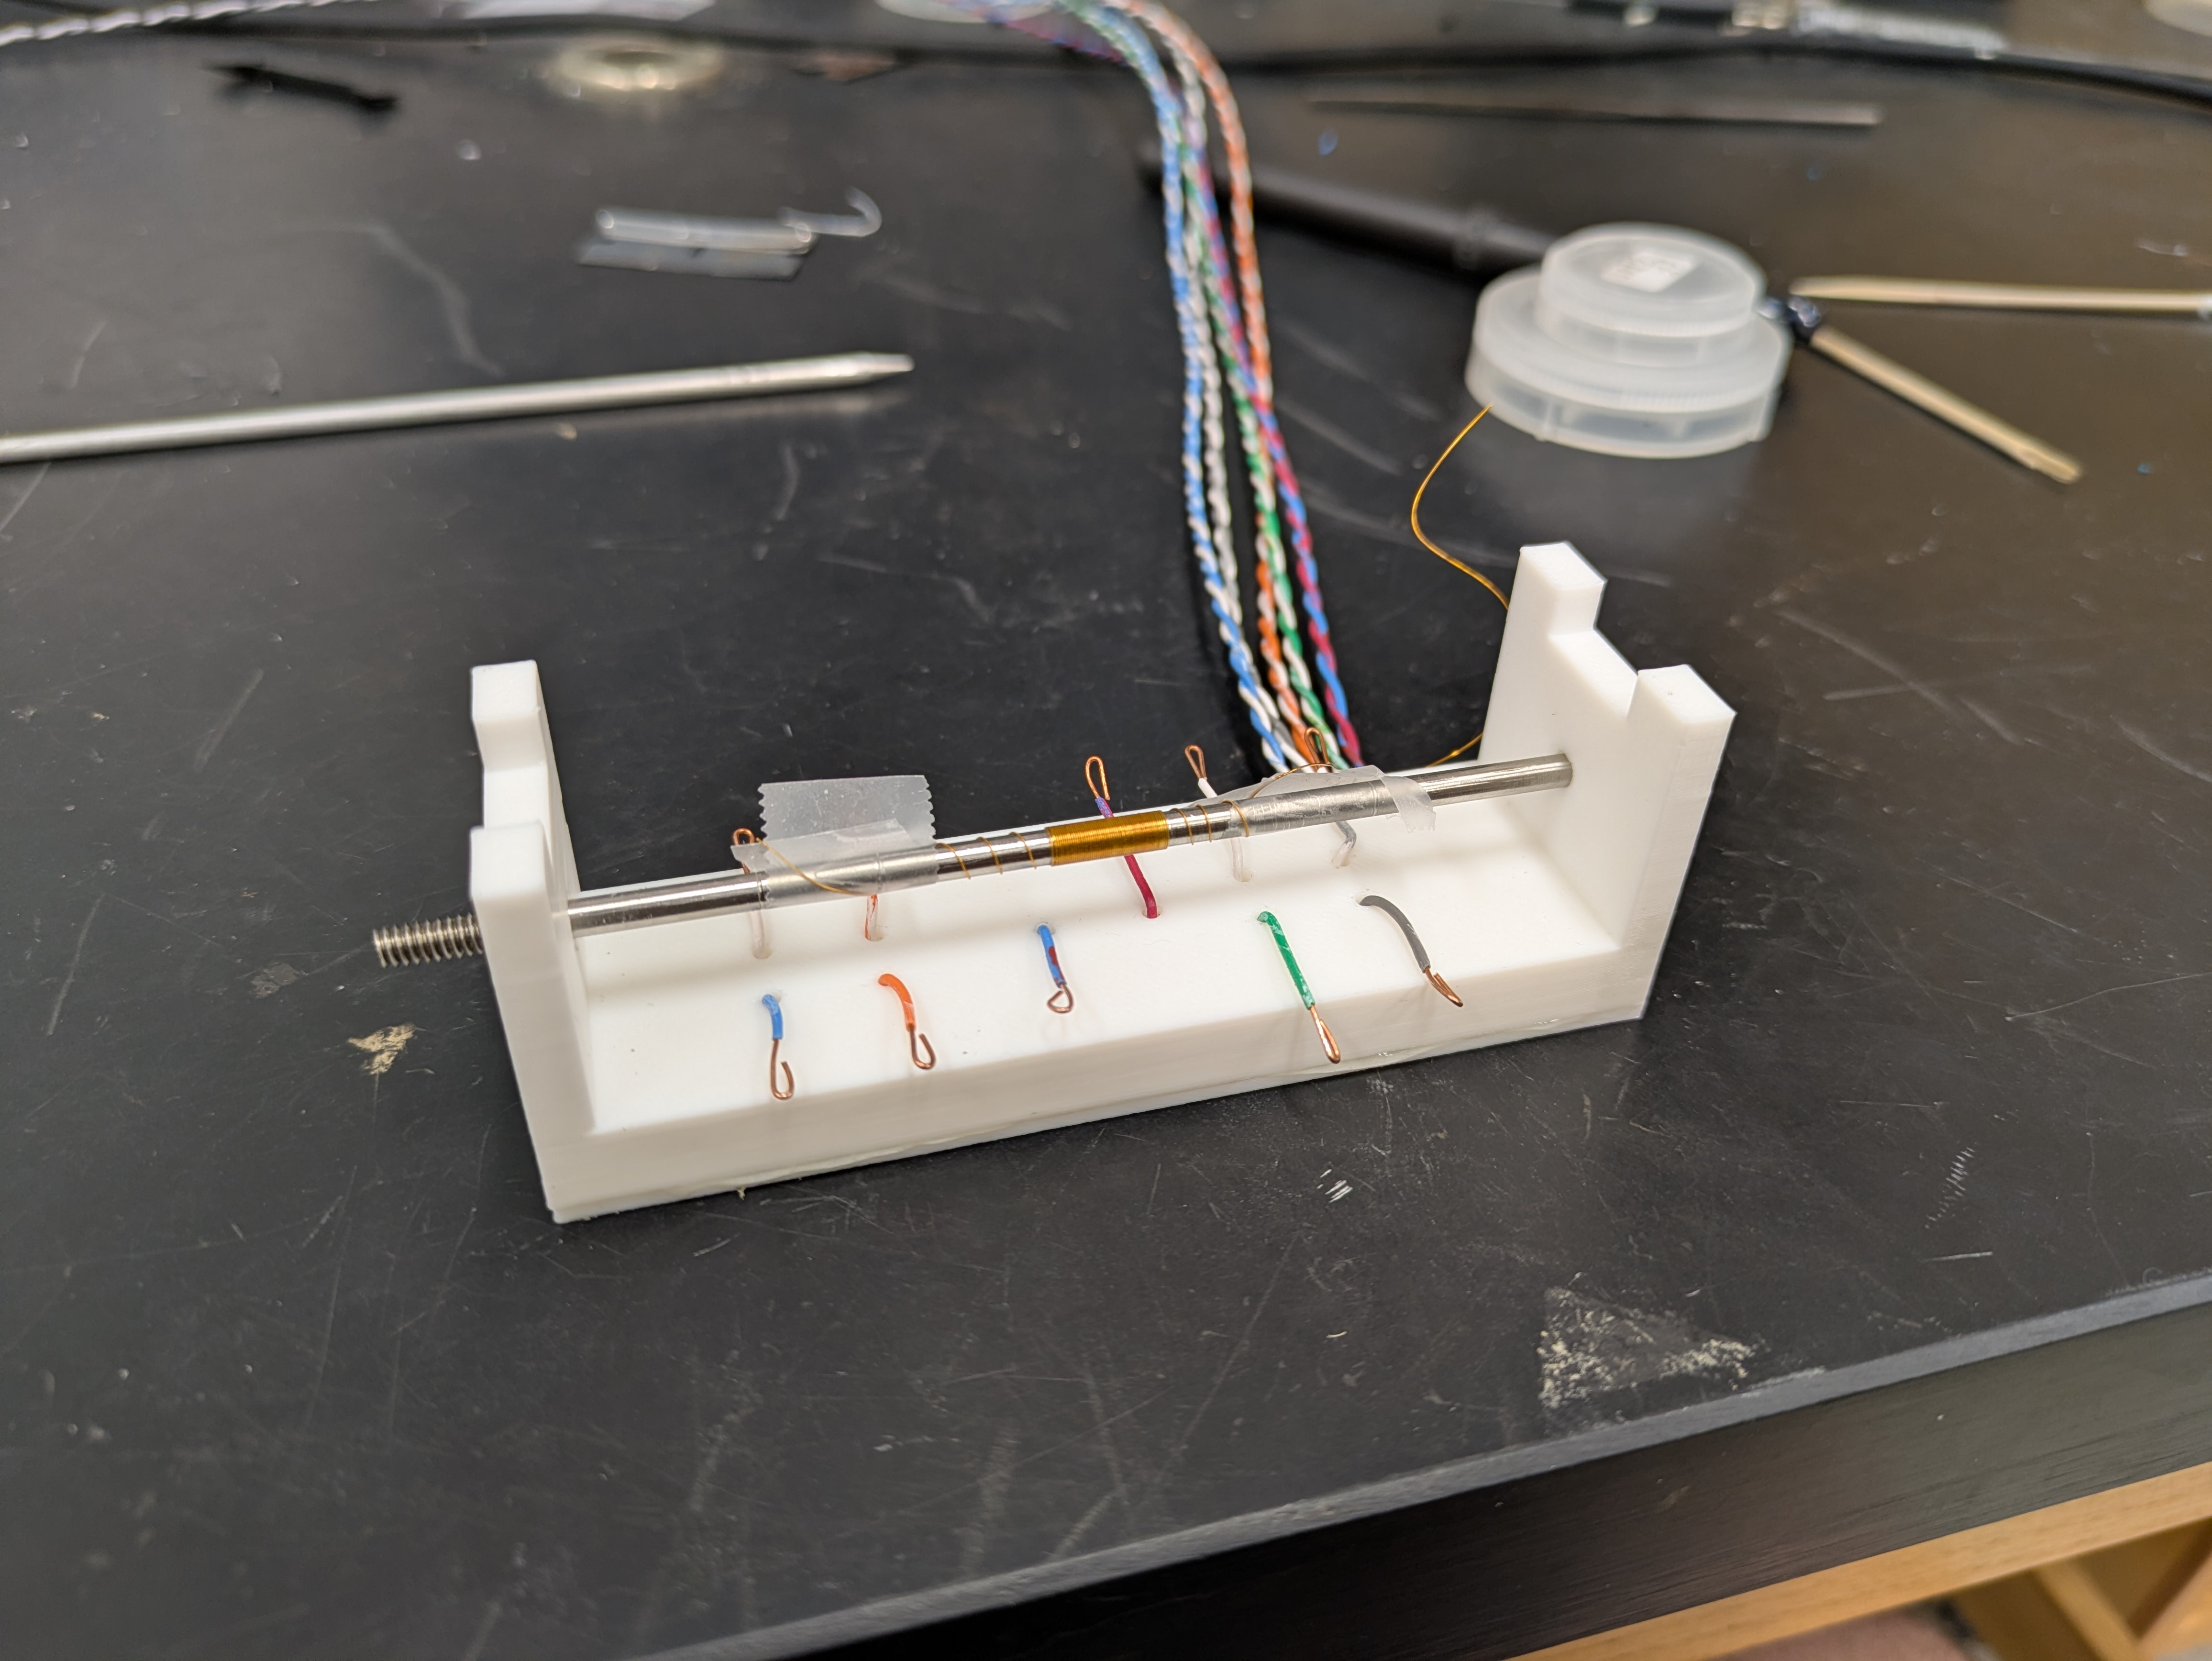
\includegraphics[width=\linewidth,trim={0 28cm 0 20cm},clip]{PXL_20260310_135734838.jpg}
		\caption{A view of the 10 cm stainless steel rod with the heater coiled prior to thermal epoxy.}
		\label{Heater full view}
	\end{figure}
	\begin{figure}[h!]
		\centering
		\begin{minipage}[c]{0.45\linewidth}
			\centering
			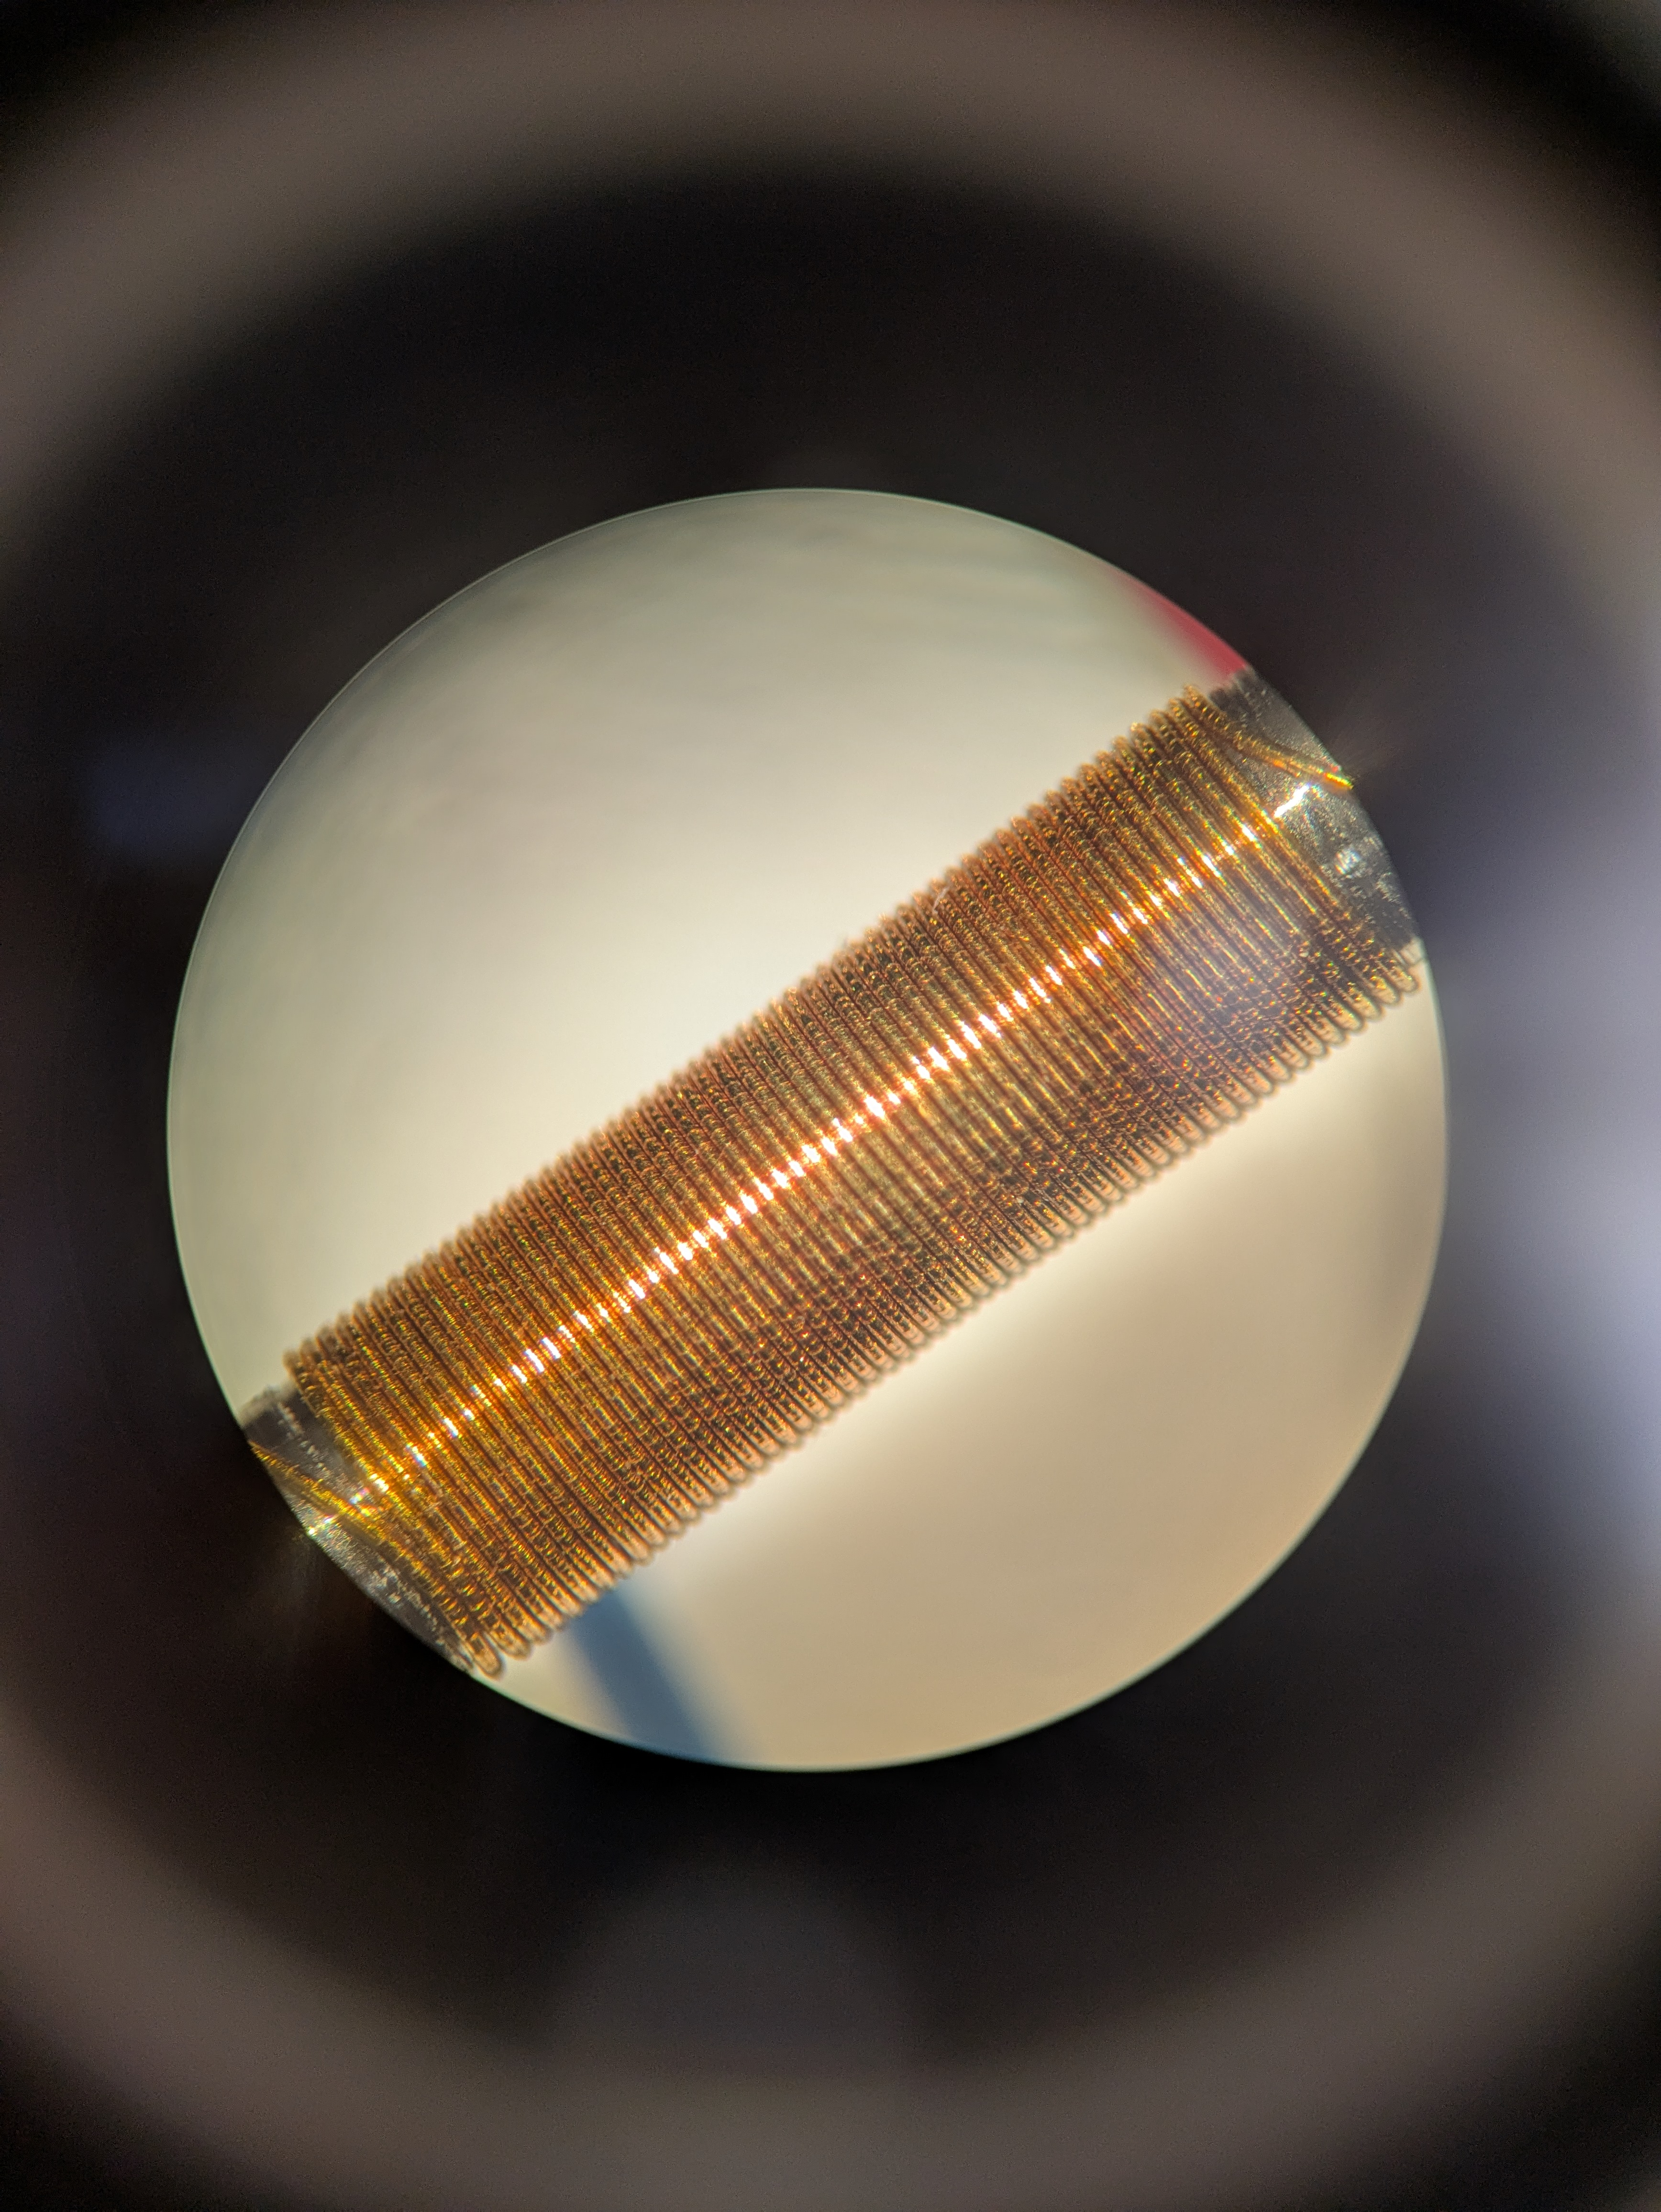
\includegraphics[
			width=\linewidth,
			trim={0 40cm 0 45cm},
			clip
			]{PXL_20260310_144003496.jpg}
			\caption{A close up of the coiled heater on the 10\,cm stainless steel rod, prior to thermal epoxy.}
			\label{fig:heater-closeup}
		\end{minipage}
		\hfill
		\begin{minipage}[c]{0.45\linewidth}
			\centering
			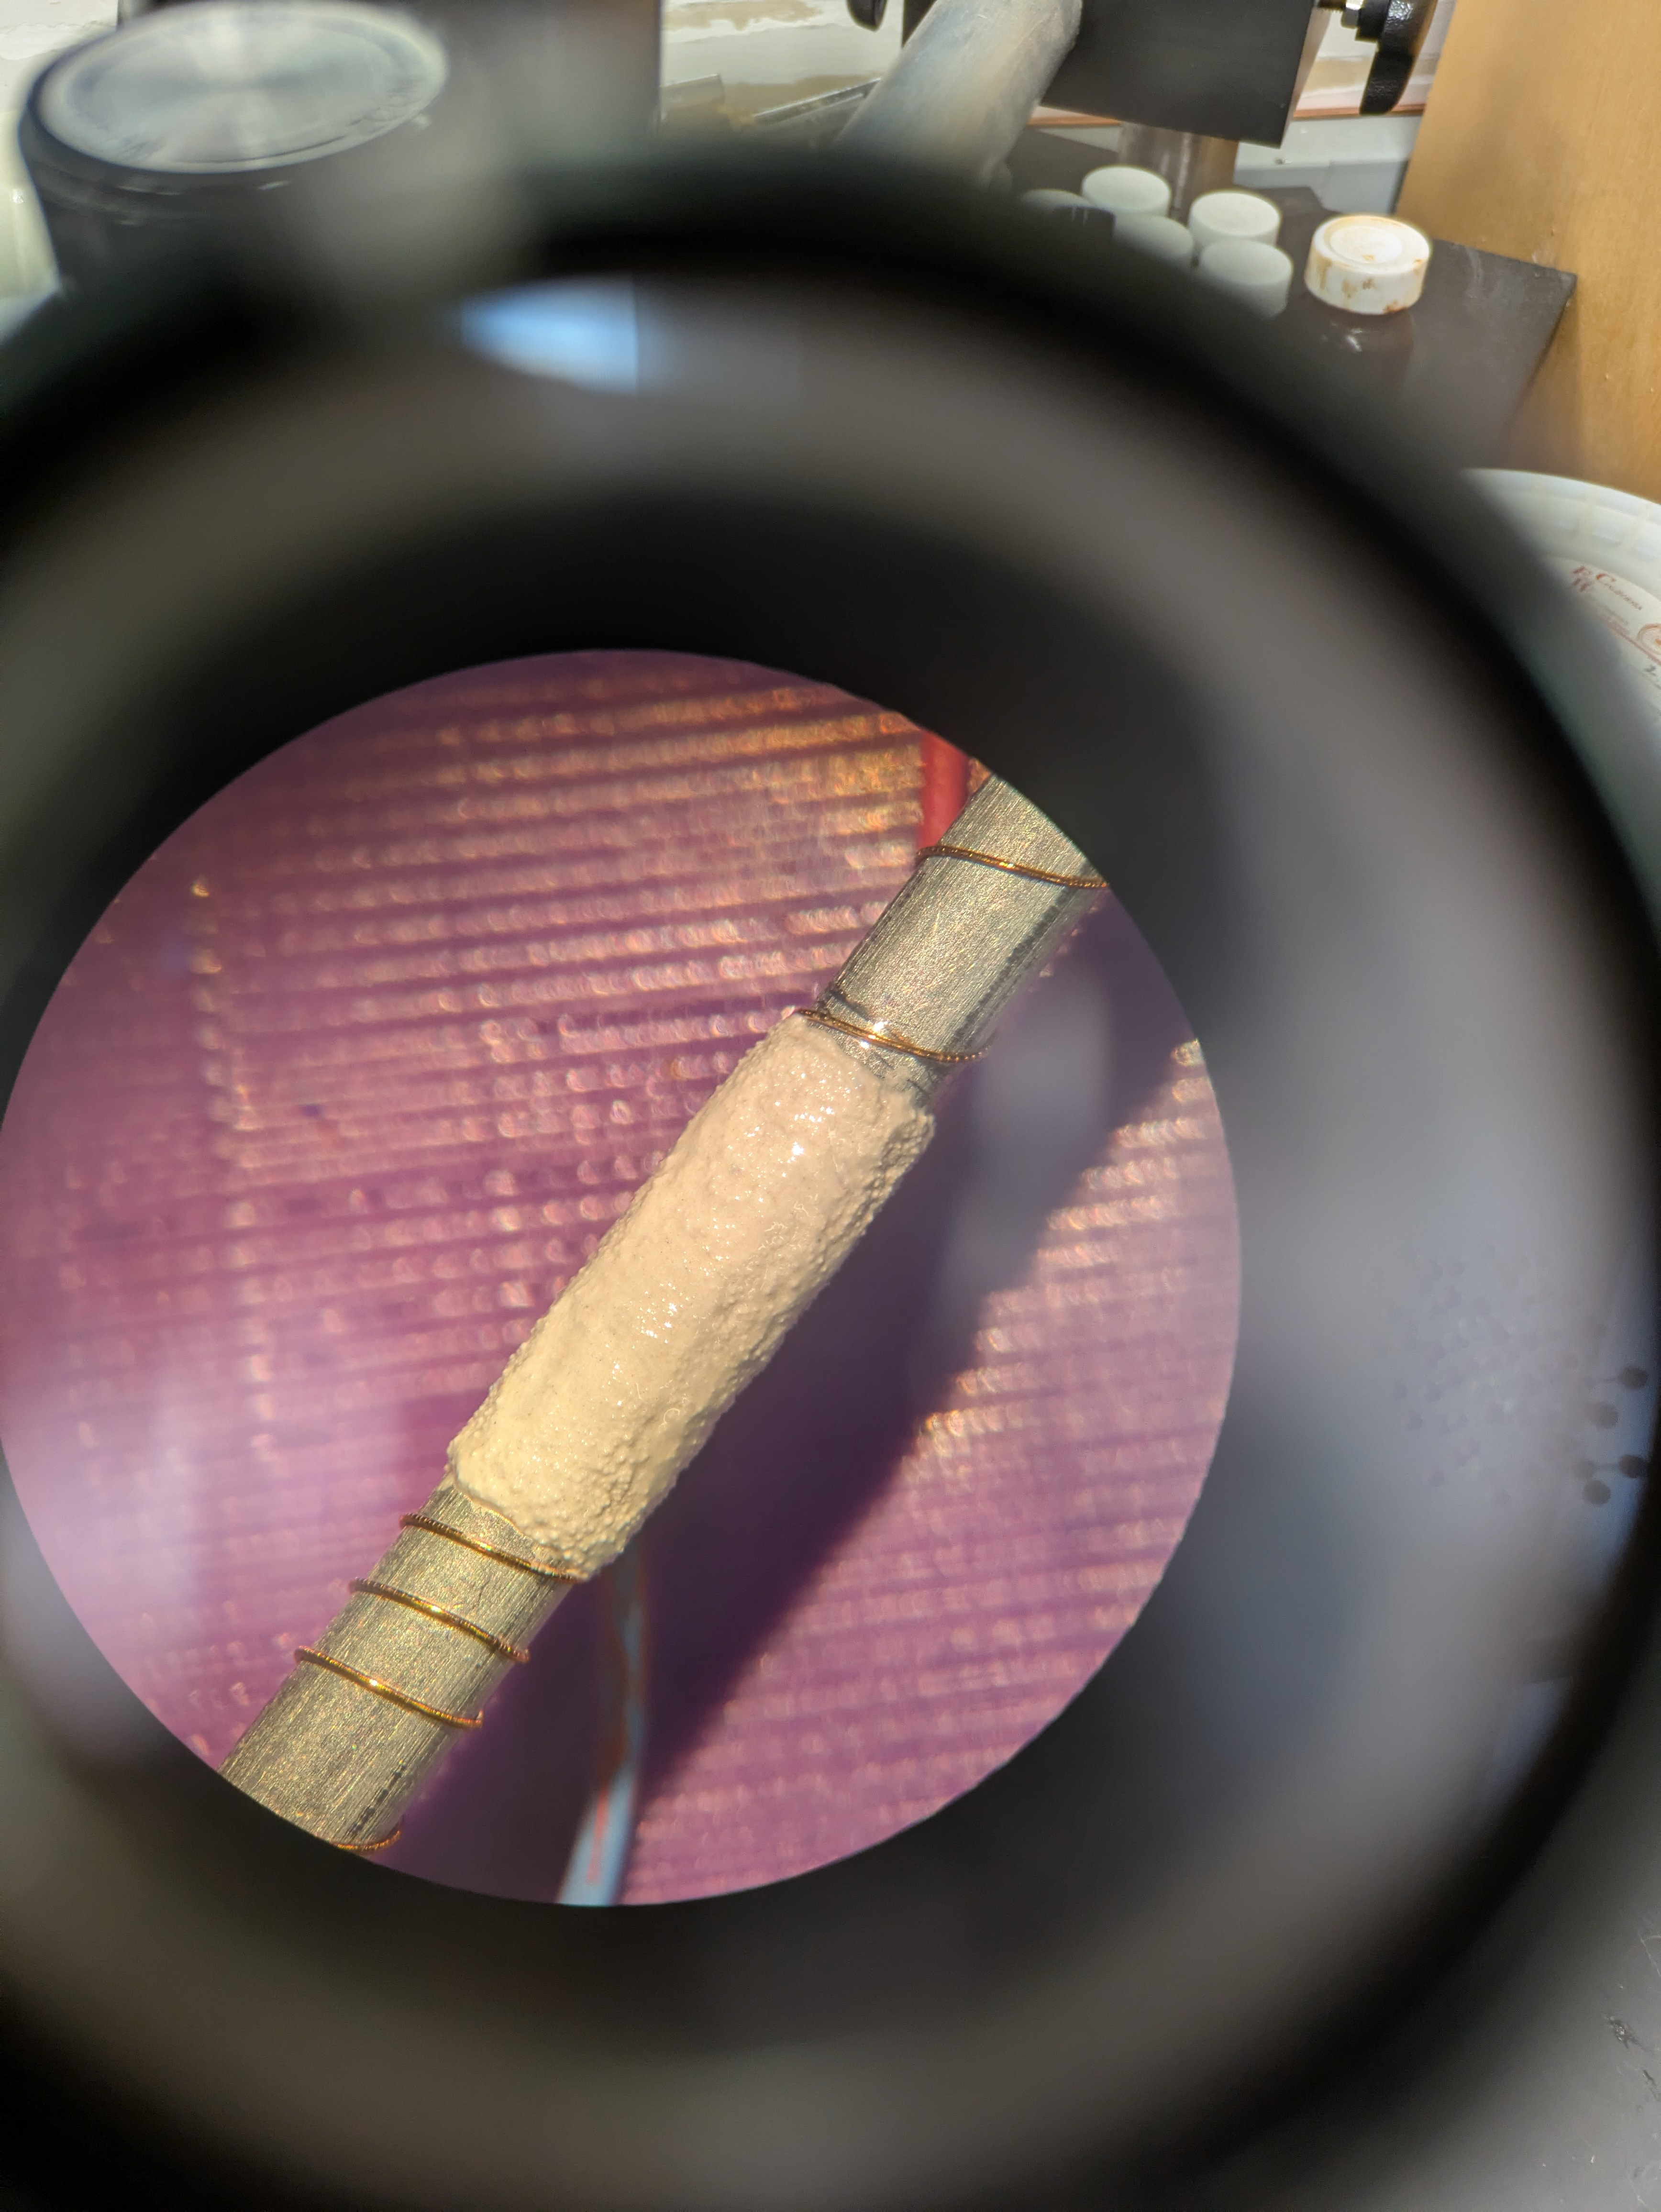
\includegraphics[
			width=\linewidth,
			trim={20cm 40cm 50cm 70cm},
			clip
			]{PXL_20260331_154734230.jpg}
			\caption{A close up of the coiled heater on the 10\,cm aluminum rod, after thermal epoxy.}
			\label{fig:epoxy-heater}
		\end{minipage}
	\end{figure}
	The next aspect that I took on was creating the heater for the rods. The heaters for these rods is simply a length of copper wire wrapped around the rod to form a coil with width of 1cm. Along this process, after re-wrapping with the same length of wire following a couple mistakes causing loss of tension, I noted some issues when examining it under the microscope. The wire that I was using to wrap and form the heater is on the older side, so upon wrapping and unwrapping repeatedly, the shielding around the wire had cracked, and in some places come off completely. Upon testing, this resulted in the heater shorting to the rod, which would not appropriately function for our purposes. Thus, I had to wrap using a length of wire not previously damaged. Images of these heaters can be seen in Figures \ref{Heater full view} and \ref{fig:heater-closeup}. After the heaters are properly coiled, they get coated in thermal epoxy. The goal is to completely seal it to the rod, while using the smallest amount possible in order to not add mass to the system. A heater sealed in thermal epoxy can be seen in Figure \ref{fig:epoxy-heater}. Then the two ends of copper wire from the heater were attached to the larger diameter wire running through the housing by soldering. At this time I noticed that the length of the heater was correct, but appeared to not be centered for the aluminum rod. The placement was based on marks made from each end of the rod respectively. Upon further examination, the rod ended up being 12.17cm instead of the intended 12cm. This factored into later when trying to fit the data, the position of the heater and length of the rod needed to be adjusted. The aluminum rod was the only one affected.
	\subsubsection{Thermistors}
	Thermistors were the next step to preparing the rod. These were attached by putting a tiny amount of the thermal epoxy onto the rod at the appropriate spot, then settling the thermistor on top of it. The thermistor was then seated more deeply in the epoxy, and more epoxy was put over top, but only just enough to cover it. During this step it was important to make sure that no part of the thermistor wire touched the rod to make sure there wouldn't be any shorting. The thermistor wires then needed to be bent and almost wrapped around the corresponding copper loop to prepare for soldering. It was also important that there be some slack on that wire, as small rotations of the rod could cause the wires to snap unless given some leniency. Then, similar to the heater, the ends of the thermistor were soldered to the corresponding copper wires that go through the housing.
	\subsubsection{Finalizing the rods}
	Before sealing the rod in the housing, the resistance of the heater was thoroughly measured. This was done by using a four point probe method, to eliminate any alterations caused by contact and lead resistance for example. The appropriate resistances were then printed in sticker form and stuck on the housings. After all the wires were appropriately soldered, the housing was covered by the final part and zip tied shut. All the thermistors were also checked again to make sure that they were still connected upon closing. The 20cm stainless steel rod did have issues when it was originally shut, and a couple of the thermistors ended up broken. The heat sinks then needed to be attached to the ends of the rod, which needed to be done more carefully than I did, as I ended up breaking all of the thermistors, requiring me to solder them back together.
	\section{Data taking}
	In order to take data, the setup was put in the vacuum chamber, and the wires for each of the appropriate elements were connected to the breadboard leading the wires outside the vacuum. The thermistors were each then tuned in order to ensure that they wouldn't hit either their top or bottom limit, and appropriately capture the data. Using MATLAB to capture data, I used a previous program developed for this, and simply adjusted the parameters such as pulse length, heater voltage, and collection length time. The data can be found in the data folder of the GitHub repository linked prior, which also includes all of the graphs I made of the different attempted fits. The only remaining part that I worked on was attempting to fit the model to the data. 
	\section{Data and analysis}
	All the data that will be discussed after this will be data taken on the 10cm aluminum rod, both sides thermally sunk. Upon beginning to fit the data I was struggling to get good agreement with the model. Some early issues presented themselves. One of the issues we ran into was the shape of the diffusion being entirely wrong, which, ended up being due to the thermal properties I had assigned the aluminum rod. In actuality we used a different type of aluminum than I had accounted for, thus fixing the shape of the graph. However, we were still left with an issue of temp peaks being significantly different. One such way this was fixed was by calculating the actual effective resistance of the heater, which ended up being 6.75$\Omega$ instead of the previous value of 5.02$\Omega$. This helped get the peak closer to the data, but there was still a difference. The next thing I noted was that since we were no longer measuring the temperature of the room while taking the data, we could have an inaccurate initial temperature of the rod, which could account for the mismatch in peak temperature. However, my previous value had been 30\degree C, and upon lowering it to the appropriate room temperature, the numerical model significantly overestimates the peak temperature. When I attempted to scale the data to the model, I found that they are all off by a factor of 0.8-0.9 times actual. This suggests that the model is accurately representing the diffusion throughout the rod, with the only difference being an issue in the amount of heat put into the system. I was unable to figure out what the cause is for that difference in my time. These graphs can be seen as Figure \ref{fig:scaled-data} and \ref{fig:unscaled-data}. Previously I mentioned that the rods needed to be treated as their whole 12cm or 22cm length in previous years, and this remained the case, as the fitting was much better using the full 12cm.
	\begin{figure}
		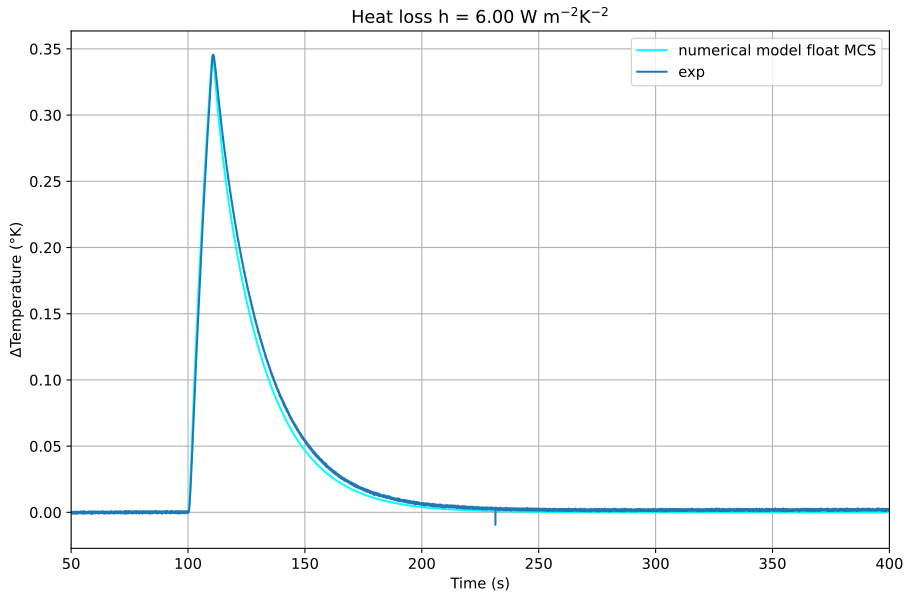
\includegraphics[width=\linewidth]{../../Data-and-Papers/2026Data/Data Fitting/10sAlfit.png}
		\caption{This graph shows the fitting of the numerical model to the actual data. In this case, the actual data has been scaled by a factor of 0.86 in order to show that the shape is proper and the difference is mostly a factor of Q.}
		\label{fig:scaled-data}
	\end{figure}
	\begin{figure}
		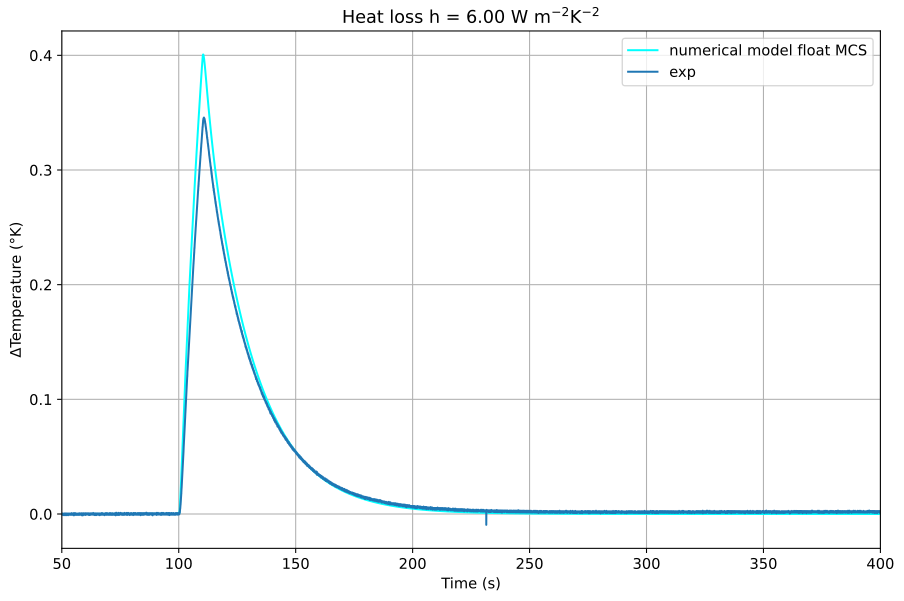
\includegraphics[width=\linewidth]{../../Data-and-Papers/2026Data/Data Fitting/10sAlnotfit.png}
		\caption{This graph shows the fitting of the numerical model to the data. This is the actual fit of the model to the data without any scaling.}
		\label{fig:unscaled-data}
	\end{figure}
	\newpage
	\section{Conclusions}
	To sum up the work I have done succinctly: I created 3 new setups to test thermal diffusion using different materials and lengths, modeled the changes, took some data, and began to fit it. This project can be continued by taking data with the other 2 setups that I was unable to get to, as well as testing different circumstances such as sunk or not, and vacuum versus open to the air. Additionally, there is more work that can be done to fit the model to the data and figure out why there is a difference in the peak temperature in our current attempted fit. Another place for further work could be optimizing the housing of the rods in an attempt to secure the rods from spinning when attaching the heat sinks.
\end{document}